
Fields are the basic data holding facilities in \libpniio\ and are represented
by instances of \nxfield. One can imagine a field as a multidimensional array 
stored on disk. Thus, it has quite similar properties than instances of 
\cpp{mdarray} in \libpnicore.  It is impossible to create a purely 
scalar field with \libpniio\ as every field should be extensible if required. 

%%%===========================================================================
\subsection{Creating fields}

Fields are created as children of a particular group instance. Creating fields
is a rather complex task as there are many options available so lets start with 
the simplest possible example
\begin{cppcode}
h5::nxgroup entry = root["entry"];
h5::nxfield field = entry.create_field<float32>("temperature");
\end{cppcode}
This creates a 1D field with a single element. This is as closest one can get 
to store a scalar value. The template parameter of the \cpp{create\_field}
method can be any type supported by \libpnicore.  For multidimensional fields
use 
\begin{cppcode}
h5::nxgroup entry = root["entry"];
h5::nxfield field = entry.create_field<float32>("temperature",shape_t{3,4});
\end{cppcode}
which will create a $2$-dimensional field with a shape of $(3,4)$ and a total
size of $12$ elements.
When using HDF5 as a storage format a compression algorithm can be associated
with a field. This algorithm will later on be used to compress the data stored
in a field and thus reduce disk utilization of the file. 
Currently only the standard deflate filter is supported 
\begin{cppcode}
h5::nxgroup entry = root["entry"];
h5::nxdeflate_filter deflate(4,false);
h5::nxfield field = entry.create_field<float32>("temperature",shape_t{3,4},deflate);
\end{cppcode}
In this particular case the filter uses a compression level of $4$ and no 
fletcher pre-sorting of the data. 

%%%===========================================================================
\subsection{Reading and writing data}

Fields provide two basic methods for reading and writing data: \cpp{read()} and
\cpp{write()}. Both member functions accept a single argument which can be an
instance of the following types
\begin{center}
    \begin{tabular}{l|p{0.6\linewidth}}
        {\bf type} & {\bf description} \\
        \hline
        \hline
        {\tt mdarray<...>} & an instance of the {\tt mdarray} template \\
        \hline
        {\tt array} & an instance of the array type erasure \\
        \hline
        {\tt T\& } & a single scalar value of the fields element type or a 
        convertible type \\
        \hline
    \end{tabular}
\end{center}
In addition there is a special version of \cpp{read()} and \cpp{write()}
available for legacy code with raw pointers. The two functions have the
signatures
\begin{cppcode}
template<typename T> void read(size_t n,T *ptr);
template<typename T> void write(size_t n,const T *ptr);
\end{cppcode}
The additional first argument \cpp{n} is the number of elements of type \cpp{T}
referenced by the pointer \cpp{*ptr}. This number ensures that the functions 
can check if the size of the field matches the number of elements which should
be read from or written to memory.
A scalar can be read from a field simply with
\begin{cppcode}
float32 temperature; 
h5::nxfield field = ...;
field.read(temperature);
\end{cppcode}
and writing runs exactly as one would expect
\begin{cppcode}
float32 temperator = ...;
h5::nxfield field = ...;
field.write(temperature);
\end{cppcode}
The same simple concept applies to all other types. For an instance of 
\cpp{mdarray} the code would look like this
\begin{cppcode}
auto data = dynamic_array<uint32>::create(shape_t{1024,1024});
h5::nxfield background = ....;

background.write(data); //writing

background.read(data);  //reading
\end{cppcode}

The \cpp{read()} and \cpp{write()} member functions perform a size check on
their arguments. The size of the argument must match the size of the field. 
In the case of scalar data a field-size of $1$ is assumed. If argument and field
size do not match a \cpp{size\_mismatch\_exception} is thrown.

%%%===========================================================================
\subsection{Growing fields}

%%%---------------------------------------------------------------------------
\begin{figure}[tb]
\centering
\begin{minipage}[c]{0.3\linewidth}
    \begin{cppcode}
h5::nxfield f = ...;
//..... code omitted ......
f.grow(0,4);
    \end{cppcode}
\end{minipage}
\hfill
\begin{minipage}[c]{0.65\linewidth}
    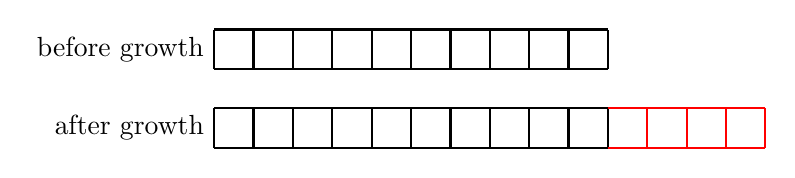
\begin{tikzpicture} [field/.style = {thick,step=5mm} ]
    \draw[field] (0mm,0mm) node[anchor = east,yshift=+2.5mm] {before growth} grid (50mm,5mm); 
    \draw[field] (0mm,-10mm) node[anchor=east,yshift=+2.5mm] {after growth} grid +(50mm,5mm);
    \draw[field,color=red] (50mm,-10mm)  grid +(20mm,5mm);
    \end{tikzpicture}
\end{minipage}
\caption{{\small\label{fig:field:growth1d} Growing a one dimensional field 
by $4$ elements.}}
\end{figure}
%%%---------------------------------------------------------------------------

%%%---------------------------------------------------------------------------
\begin{figure}[tb]
    \begin{minipage}[c]{0.3\linewidth}
        \begin{cppcode}
h5::nxfield f = ...;
//..... code omitted .....
f.grow(1,4);
        \end{cppcode}
    \end{minipage}
    \hfill
    \begin{minipage}[c]{0.65\linewidth}
        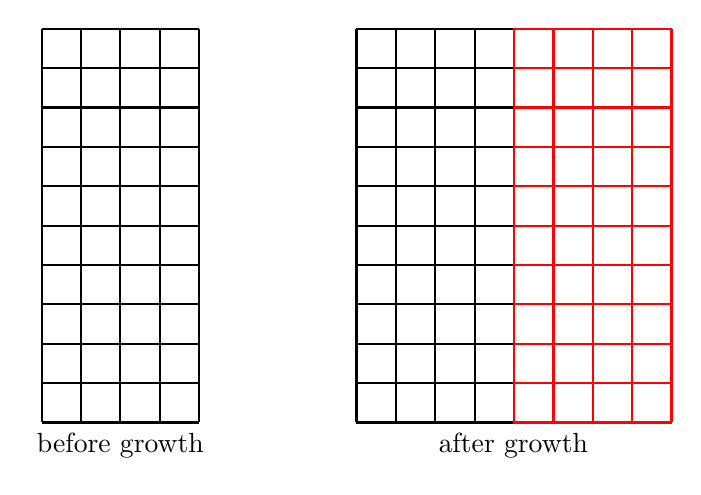
\begin{tikzpicture} [field/.style = {thick,step=5mm} ]
        \draw[field] (0mm,0mm) node[anchor = north,xshift=10mm] {before growth} grid (20mm,50mm); 
        \draw[field] (39.9mm,0mm) node[anchor=north,xshift=20mm] {after growth} grid +(20mm,50mm);
        \draw[field,color=red] (59.9mm,0mm)  grid +(20.1mm,50mm);
        \end{tikzpicture}
    \end{minipage}
    \caption{{\small\label{fig:field:growth2d} Growing a two dimensional field
    by $4$ elements along its second dimension.}}
\end{figure}
%%%---------------------------------------------------------------------------
The reason why there are no purely scalar fields is that during an experiment 
one would append data to a field as the measurement progresses. 
For this purpose \nxfield\ provides a \cpp{grow()} method which allows to 
extend the field along a particular dimension. The member function has the 
signature
\begin{cppcode}
void grow(size_t e,size_t n=1)
\end{cppcode}
where the first (mandatory) argument is the index of the dimension along which
the field should grow and the second (optional) argument contains the number of 
elements by which to grow. Figures~\ref{fig:field:growth1d} and
\ref{fig:field:growth2d} show examples of growing a one and a two dimensional
field respectively.

The canonical application for this feature would be to add content to a field 
as an experiment progresses. Using such a pattern we can start with a field 
of $0$ size and then add points if required. The principal code would look like
this
\begin{cppcode}
h5::nxfile f = ...;
h5::nxfield data = detector_group.create_field<uint16>("spectra",
                                                       shape_t{0,1024});
size_t index = 0;
while(true)
{
    data.grow(0,1); //grow by one element along first dimension
    //...... code omitted ....
}
\end{cppcode}
Note here that the initial shape of the field is $(0,1024)$. Such a pattern 
removes the burden of determining the number of points, recorded during 
an experiment, before the experiment starts. If the measurement is stopped 
somewhere in between the number of points written to the file matches exactly
the number of points recorded.  
It is important to note that one cannot extend the size of a field only along
\emph{existing} dimensions. It is not possible to change the rank of a field via
the growth method. Every attempt to do so will raise an \cpp{index\_error}
exception.
How to write the data will be explained in the next section.

%%%===========================================================================
\subsection{Partial reading and writing}

The previous section explained how to adjust the size of fields dynamically. 
What is still missing is how to write data to such a growing field. The 
\cpp{read()} and \cpp{write()} member functions used so far are always writing
the entire content of the field. This is not really what we want. 
Thus, \libpniio s \nxfield\ type provides partial IO quite similar to the 
\cpp{mdarray} template of \libpnicore. 

The best way to understand partial IO is to have a look on an example. We thus
will complete the previous one 

\begin{cppcode}
h5::nxfile f = ...;
h5::nxfield data = detector_group.create_field<uint16>("spectra",
                                                       shape_t{0,1024});
auto buffer = dynamic_array<uint16>::create_array(shape_t{1024});

size_t index = 0;
while(true)
{
    data.grow(0,1); //grow by one element along first dimension
    //...... code omitted ....

    //write data
    data(index++,slice(0,1024)).write(buffer);
}
\end{cppcode}
The important line of code here is the last one in the \cpp{for}-loop. To obtain
a selection of a field we can use the \cpp{()} operator of \nxfield. 
The selection works the same as for \cpp{mdarray}. However, the return value is 
a new field instance with the selection set. One currently cannot apply more
selections successively. 


%%%===========================================================================
\subsection{Field inquiry}

Fields share a set of inquiry functions with groups. These are \cpp{name()}, 
\cpp{filename()}, and \cpp{is\_valid()}. In addition to these functions
there are also some member functions which are special for fields. 
The \cpp{size()} member function returns the total number of elements 
stored in a field. If a selection has been applied to the field \cpp{size()}
returns the total number of elements selected. 
\cpp{type\_id()} returns the Id of the field elements data type. 
The \cpp{shape()} template function returns a container, which can be passed as
a template parameter, with the number of elements along each dimension. 
\begin{cppcode}
h5::nxfield field = ...;
auto s = field.shape<shape_t>();
\end{cppcode}
